\label{chapter:improvements}

In this chapter we look at two improvements to the binary XPFC theory. Both of
these improvements are novel contributions to the field and significantly
extend the scope of the XPFC framework. The improvements, as previously alluded
to, are to first, extend the free energy of mixing in the XPFC model to one
with an enthalpy of mixing and to second, generalize the phenomenological
for of the two-point correlation function in binary alloys.

%%%%%%%%%%%%%%%%%%%%%%%%%%%%%%%%%%%%%%%%
\section{Adding an Enthalpy of Mixing} %
%%%%%%%%%%%%%%%%%%%%%%%%%%%%%%%%%%%%%%%%

Extending the free energy of mixing beyond ideal mixing is achieved by removing
the assumption made by Greenwood \textit{et al.} in deriving the binary XPFC
model that the concentration-concentration correlation function has no $k=0$
mode. This is the same approach taken in the original PFC model, though here we
keep the ideal mixing term unexpanded as in the original XPFC alloy model.
Specifically, the correlation function is expanded as,
%
\begin{equation}
    C_{cc}(r, r^\prime) = \d(r - r^\prime)
        \l(\omega\epsilon + W_c\nabla^2 + \cdots\r),
\end{equation}
%
where $\epsilon$ is a parameter that is possibly temperature dependent. This
form results in a free energy functional of the form,
%
\begin{align}
    \f{\beta\Delta\F[n, c]}{\rho_0} &= \integrate{r} \l\lbrace
        \f{1}{2} n(r) \l(1 - C_{nn}(r, r^\prime)\r) \ast n(r^\prime)
        - \eta \f{n^3}{6} + \chi \f{n^4}{12} \r\rbrace \\
        &+ \integrate{r}\l\lbrace
            \f{W_c}{2}\l\vert \nabla c(r) \r\vert^2 + \omega f_{mix}(r)
            \r\rbrace, \nonumber
\end{align}
%
where the local free energy density of mixing, $f_{mix}$ is now,
%
\begin{equation}
    f_{mix}(r) = \l(n(r) + 1\r)\l(
            c(r)\ln\l(\f{c(r)}{c_0}\r)
          + (1-c(r))\ln\l(\f{1-c(r)}{1-c_0}\r) \r)
          + \f{1}{2} \epsilon (c - c_0)^2.
\end{equation}
%
For simplicity the temperature dependence of the parameter $\epsilon$ is taken
to be linear about a spinodal temperature $T_c$,
%
\begin{equation}
    \label{eq:spinodal_model}
    \epsilon(T) = -4 + \epsilon_0(T - T_c).
\end{equation}
%
The resulting model has a free energy of mixing that is equivalent to the
regular solution model and, as such, it makes a clear connection to a well used
model elsewhere in material science. The regular solution model also supplies
the essential physics of a non-negligible enthalpy of mixing. 

%%%%%%%%%%%%%%%%%%%%%%%%%%%%%%%%%%%%%%%%%%%%%%%%%%%%%%%%%%%
\section{Generalizing the Two-Point Correlation Function} %
%%%%%%%%%%%%%%%%%%%%%%%%%%%%%%%%%%%%%%%%%%%%%%%%%%%%%%%%%%%

To establish a general phenomenology for modelling density-density correlation
functions in alloys, note that the density-density correlation function has the
form of a linear combination of interpolating functions in concentration,
$\zeta(c)$, multiplied by bare correlation functions $C(r, r^\prime)$ of
individual components,
%
\begin{equation}
    C_{nn}(r, r^\prime; c) = \sum_i \zeta_i(c) C_i(r, r^\prime)
\end{equation}
%
where the index $i$ is, for the moment, an arbitrary label. For example, in the
exact theory that emerges from the original alloy CDFT theory (equation
\ref{binaryCs}), we use the labels $\lbrace AA, AB, BB\rbrace$ and have
interpolation functions,
%
\begin{gather}
    \zeta_{AA}(c) = \rho_0 (1 - c^2), \\
    \zeta_{AB}(c) = \rho_0 c (1 - c ), \\
    \zeta_{BB}(c) = \rho_0 c^2.
\end{gather}
%
This suggests the following new definition that we introduce herein to
generalizethe density-density correlation function for a binary alloy: Use the
labels $i$ to enumerate the set of crystal structures known to manifest
themselves in an alloy system. The correlation functions, $C_i(r, r^\prime)$
are then direct correlation functions that model the crystal structure $i$ and
the associated interpolation functions $\zeta_i(c)$ define the range of
concentrations over which these correlations are valid. In principle,
$\zeta_i(c)$ can also be temperature dependent, although we do not consider
that case in this thesis.

As a simple example, if we wanted to construct a model of the silver-copper
eutectic alloy system, we might start with some model correlation function for
pure silver, $C_\alpha(r, r^\prime)$, and for pure copper, $C_\beta(r,
r^\prime)$. These two structures, the silver rich $\alpha$ phase and the copper
rich $\beta$ phase, are the only two relevant crystalline phases in the system,
so to build the full density-density correlation function we just need to
choose interpolating functions for each phase. Following Greenwood \textit{et
al} for example, we might choose,
%
\begin{gather}
    \zeta_\alpha(c) = 1 - 3c^2 + 2c^3, \\
    \zeta_\beta(c) = 1 - 3 (1 - c)^2 + 2(1 - c)^3.
\end{gather}
%
To model the $\alpha$ and $\beta$ correlation functions we use the original
XPFC formalism for modelling bare correlation functions (i.e. equation
\ref{XPFC_C2}). The $\alpha$ and $\beta$ phase are both FCC
\cite{SUBRAMANIAN93} so we can use an FCC model for the correlation function as
in \cite{GREENWOOD10}.

%%%%%%%%%%%%%%%%%%%%%%%%%%%%%%%%%%%%%%%%%%%%%%%%%%%
\section{Equilibrium Properties of Binary Alloys} %
%%%%%%%%%%%%%%%%%%%%%%%%%%%%%%%%%%%%%%%%%%%%%%%%%%%

These two changes to the XPFC formalism extend the possible systems we can
study. In this section we'll explore the equilibrium properties of the improved
XPFC free energy functional specialized for three different material phase
diagrams: eutectic, syntectic and monotectic.

%%%%%%%%%%%%%%%%%%%%%%%%%%%%%%%%%%%%%
\subsection{Eutectic Phase Diagram} %
%%%%%%%%%%%%%%%%%%%%%%%%%%%%%%%%%%%%%

While previous PFC models have shown that elastic energy is a sufficient
driving force for eutectic solidification, our simplified regular solution XPFC
model allows for the examination of the role enthalpy of mixing can play in
eutectic solids.  For instance, Murdoch and Schuh noted that in nanocrystalline
binary alloys, while a positive enthaply of segregation can stabilize against
grain growth via solute segregation at the grain boundary, if the enthaply of
mixing becomes too large this effect can be negated by second phase formation
or even macroscopic phase separation\cite{MURDOCH13}. 

To specialize our simplified regular model to the case of the binary eutectic,
we must choose an appropriate model for the correlation function. Choosing an
$\alpha$ phase around $c = 0$ and $\beta$ phase around $c = 1$, we can recover
the pair correlation function used in the binary XPFC of Greenwood \textit{et
al.} with a particular choice of interpolations functions: 
%
\begin{align}
   \zeta_\alpha(c) &= 2c^3 - 3c^2 + 1 \\
   \zeta_\beta(c) &= \zeta_\alpha(1 - c).
\end{align}
%
Should we choose, for example, an $\alpha$ and $\beta$ phase with 2 dimensional
hexagonal lattices, differing only by lattice constants, we can produce a phase
diagram like that in Fig. \ref{eutectic}. The phase diagram also depicts the
phase diagram of the metastable liquid below the eutectic point showing the
binodal and spinodal lines where the metastable liquid becomes unstable with
respect to phase separation. The spinodal line indicates an inflexion point in
the free energy of the metastable liquid where the liquid becomes fully
unstable with respect to phase separation whereas the binodal line indicates
the coexistance curve of the decomposed metastable liquid.

\begin{figure}[h]
    \centering	
    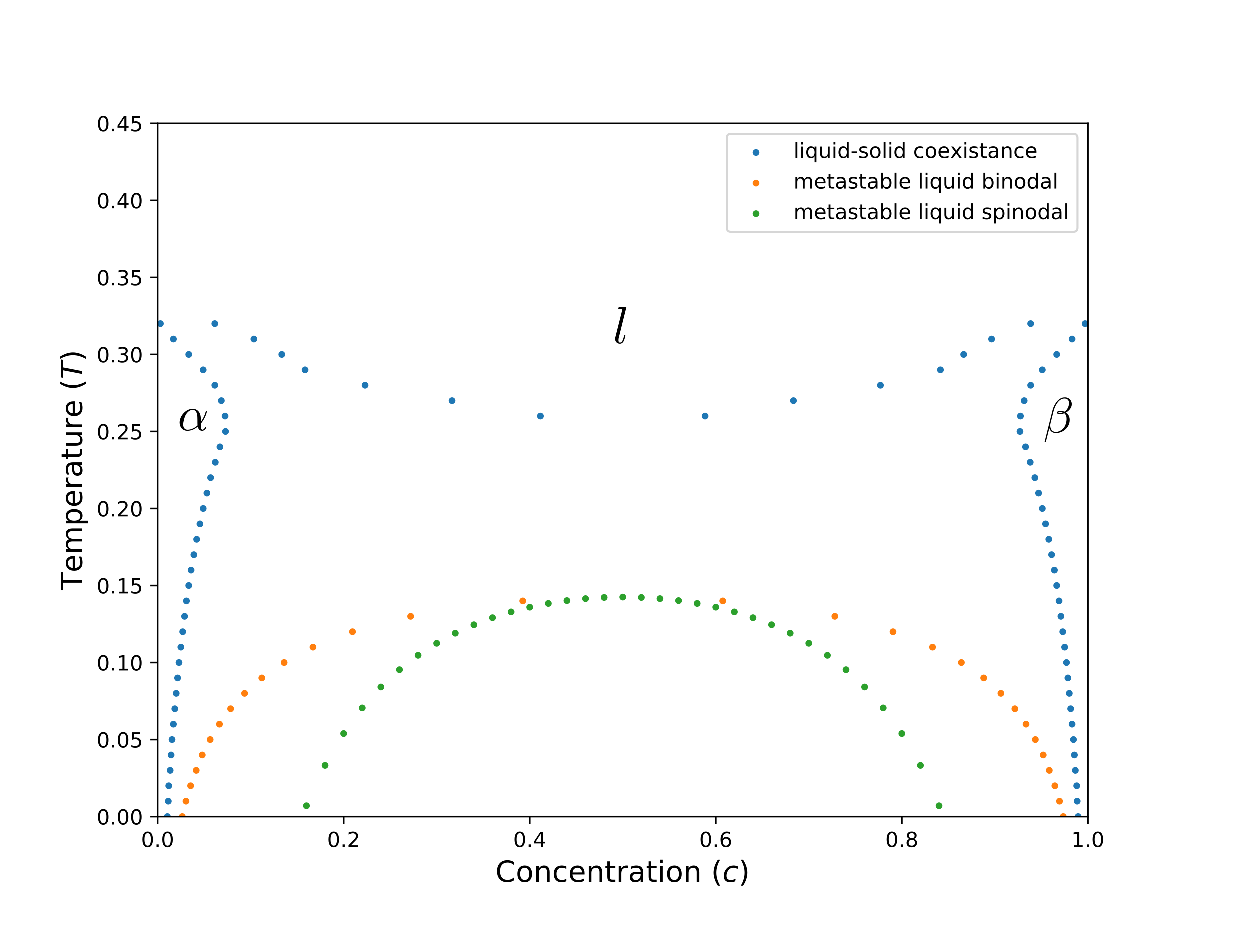
\includegraphics[scale=0.7]{eutectic}
    \caption[Eutectic Phase Diagram]{
        \label{eutectic} Eutectic phase diagram for triangle $\alpha$ and
        $\beta$ solid phases and $l$ denotes the liquid. The free energy
        parameters are $\eta = 2$, $\chi = 1$, $\omega=0.02$, $\epsilon_0 =
        26.6$ and $T_c = 0.15$. The parameters of the structure functions are
        $\sigma_{10\alpha} = \sigma_{10\beta} = 0.8$, $k_{10\alpha} = 2\pi$,
        $k_{10\beta} = 4\pi/\sqrt{3}$ and $T_0 = 1$. The horizontal line
        denotes the eutectic temperature.
    }
\end{figure}

It is noted that the phase diagram in Fig. \ref{eutectic} and in what follows
were done using the same approach that was used in numerous PFC literature
\cite{GREENWOOD11_BINARY}. The approach is as follows: a mode expansion for the
density is assumed for each crystal phases (zero amplitudes for the liquid
phase). For each  phase, an amplitude equation analogous to equation
\ref{amplitude_gp} results, except in this case, it is a function of
amplitudes, average density {\it and} concentration. This coarse grained free
energy of each phase is then minimized with respect to the amplitudes, leaving
a free energy density for each phase that is a function only of the average
density and concentration. At this juncture, we simplify matters by assuming
that the average density is a constant for the system. We then minimize the
total free energy of the system with respect to concentration, assuming a
conserved total concentration field. This latter step considers separately the
coexistence of  (1) $\alpha$-liquid, (2)  $\beta$-liquid, (3) $\alpha$-$\beta$
over different temperature/concentration ranges. Original code was developed to
carry our these phase diagram constructions, and implemented using
\texttt{Julia} \cite{JULIA}, \texttt{Maxima.jl} \cite{MAXIMAJL} and the
\texttt{Maxima} symbolic computation engine \cite{MAXIMA}.  

%%%%%%%%%%%%%%%%%%%%%%%%%%%%%%%%%%%%%%
\subsection{Syntectic Phase Diagram} %
%%%%%%%%%%%%%%%%%%%%%%%%%%%%%%%%%%%%%%

Our improved XPFC model also allows for the study of a variety of invariant
binary reactions that, to date, have not been studied using phase field crystal
models. One such reaction is the syntectic reaction. 

The syntectic reaction, $l_1 + l_2 \rightarrow \alpha $, consists of
solidification at the interface of two liquids. We can achieve this with our
model by setting the spinodal temperature, $T_c$, in equation
\ref{eq:spinodal_model} sufficiently high and producing a density-density
correlation function that is peaked at a concentration below the spinodal. This
can be done by choosing a single interpolation function to be a window 
function that is centered about an intermediate concentration, $c_\alpha$ of 
the solid phase, $\alpha$. One obvious choice is, 
%
\begin{equation}
  \zeta(c) = e^{- \f{(c - c_\alpha)^2}{2 \alpha_c^2}}
\end{equation}
%
The resulting correlation function for a hexagonal lattice in a syntectic alloy
in two dimensions becomes, 
%
\begin{equation}
  \tilde{C}_{nn}(k; c) = 
    e^{-\f{(c - c_\alpha)^2}{2 \alpha_c^2}}
    e^{-\f{T}{T_0}} 
    e^{-\f{(k - k^\prime)^2}{2\alpha^2}}
\end{equation}
%
A phase diagram that produces a syntectic reaction with an appropriate choice
of parameters can be seen in Fig. \ref{syntectic}.

\begin{figure}
    \centering
	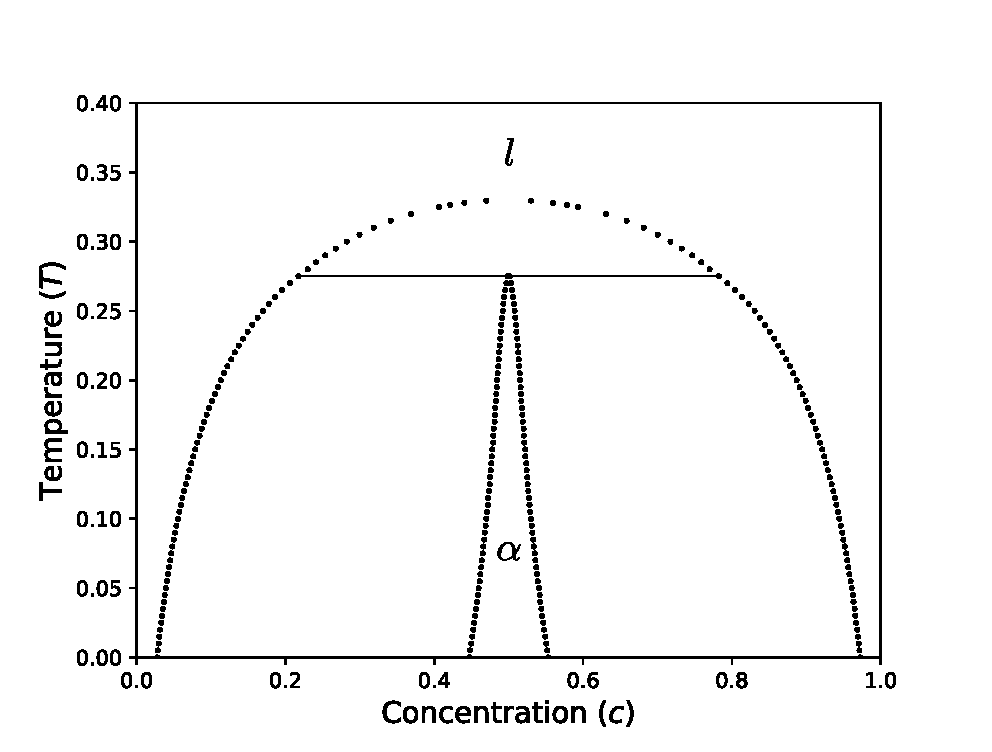
\includegraphics[scale=0.7]{syntectic.eps}
    \caption[Syntectic Phase Diagram]{
        \label{syntectic} Phase Diagram of Syntectic Alloy with a hexagonal
        solid phase $\alpha$. The free energy parameters are $\eta=2$,
        $\chi=1$, $\omega=0.3$, $\epsilon_0 = 10$ and $T_c=0.35$. The
        parameters for the structure function are $\alpha_{10\alpha} = 0.8$,
        $k_{10\alpha} = 2\pi$ and $T_0 = 1$. The horizontal line denotes the
        syntectic temperature.
    }
\end{figure}

%%%%%%%%%%%%%%%%%%%%%%%%%%%%%%%%%%%%%%%
\subsection{Monotectic Phase Diagram} %
%%%%%%%%%%%%%%%%%%%%%%%%%%%%%%%%%%%%%%%

The monotectic reaction is another invariant binary reaction that has not
previously been studied using PFC models. The monotectic reaction, $l_1
\rightarrow \alpha + l_2$, consists of decomposing liquid into a solute poor
solid and solute rich liquid. To model a monotectic using our improved XPFC
model we hypothesize a solid phase at $c=0$ and set the spinodal temperature
higher than the solidification temperature. To achieve this, we use a window
function peaked around $c = 0$,
%
\begin{equation}
    \chi_\alpha(c) = e^{-\f{c^2}{2\alpha_c^2}}.
\end{equation}
%
Again considering a simple hexagonal lattice for the $\alpha$ phase, we can
produce a phase diagram with a monotectic reaction with an appropriate choice
of parameters as in Fig. \ref{monotectic}.

\begin{figure}
    \centering
	\includegraphics[scale=0.7]{monotectic.eps}
    \caption[Monotectic Phase Diagram]{
        \label{monotectic} Phase Diagram of Monotectic Alloy with hexagonal
        $\alpha$ phase. The free energy parameters are $\eta = 2$, $\chi=1$,
        $\omega=0.3$, $\epsilon_0 = 10$, $T_c = 0.35$ and $c_0 = 0.75$. The
        parameters for the structure function are $\alpha_{10\alpha} = 0.8$,
        $k_{10\alpha} = 2\pi$ and $T_0 = 1$ and the parameter for the window
        function is $\alpha_c = 0.4$. The horizontal line indicates the 
        monotectic temperature.
    }
\end{figure}

The improvements to the XPFC formalism made in this chapter not only reveal new
details in existing systems, but also model new systems that haven't been
explored with PFC methods before. They provide a general framework to explore
the landscape of other possible possible binary alloys with an emphasis that
the liquid free energy is a crucial element in this complete description. It is
also noteworthy that the approach introduced here is extendable in a
straightforward way to multi-component alloys if the interpolation functions
become multivariate functions of the concentrations.

